\chapter{Pruebas y resultados}
%intro

\section{Pruebas parciales del módulo de registración}
%del capítulo de desarrollo
	Se realizaron pruebas preliminares de los métodos de alineación inicial
	de \emph{sample consensus} y búsqueda de \emph{clustering}
	sobre los objetos \texttt{happy} y \texttt{bunny}.
	Las capturas de \texttt{happy} se realizaron a intervalos de ángulos equiespaciados (cercanos a $24^{\circ}$) y
	presentan zonas suaves en la base, barriga y espalda.
	En cambio los ángulos en \texttt{bunny} son más variados y espaciados, yendo desde $35^{\circ}$ hasta $90^{\circ}$,
	y se observa una superficie más irregular por todo el cuerpo (figura~\ref{fig:stanford_models}).%\TODO{Sacar foto a los modelos}

	%SAC-IA
	En el caso de la alineación mediante \emph{sample consensus},
	se obtuvieron buenos resultados en la mayoría de las capturas de \texttt{happy}
	donde los ángulos eran cercanos a $25^{\circ}$ (figura~\ref{fig:dif_rot_happy}). \TODO{mentira, falló en una con happy}

	Pero al utilizar el modelo \texttt{bunny}, cuyos ángulos eran cercanos a $45^{\circ}$,
	se obtuvo una buena alineación en el caso de las capturas 315--000 y 000--045,
	sin embargo, para los otros casos las correspondencias fueron completamente erróneas (figura~\ref{fig:align_sac}).

	%Clustering
	Para el algoritmo de \emph{clustering}, en cambio,
	no se tuvieron problemas con el modelo \texttt{bunny},
	a pesar de presentar saltos cercanos a $90^{\circ}$ en las alineaciones
	contra la captura \texttt{bun180}. Si bien este salto supera las restricciones impuestas,
	en ningún caso se produjo una diferencia mayor a $5^{\circ}$ respecto al \emph{ground truth} (figura~\ref{fig:clust_bunny}).

	Para el modelo \texttt{happy} se obtuvieron resultados similares a pesar de que en este
	caso los ángulos eran más cercanos (aproximadamente $24^{\circ}$).  Las
	diferencias respecto al \emph{ground truth} no superaban los $5^{\circ}$,
	teniendo un error promedio de $2^{\circ}$ (figura~\ref{fig:dif_rot_happy}).

	De esta forma, se logró acercar las capturas lo suficiente como
	para intentar alinearlas por ICP.

\begin{figure}
	\begin{tikzpicture}[gnuplot]
%% generated with GNUPLOT 5.4p0 (Lua 5.4; terminal rev. Jun 2020, script rev. 114)
%% Tue 25 Aug 2020 01:55:33 AM -03
\gpmonochromelines
\path (0.000,0.000) rectangle (12.500,8.750);
\gpcolor{color=gp lt color border}
\gpsetlinetype{gp lt border}
\gpsetdashtype{gp dt solid}
\gpsetlinewidth{1.00}
\draw[gp path] (1.320,0.985)--(1.500,0.985);
\draw[gp path] (11.947,0.985)--(11.767,0.985);
\node[gp node right] at (1.136,0.985) {$0$};
\draw[gp path] (1.320,1.813)--(1.500,1.813);
\draw[gp path] (11.947,1.813)--(11.767,1.813);
\node[gp node right] at (1.136,1.813) {$0.5$};
\draw[gp path] (1.320,2.642)--(1.500,2.642);
\draw[gp path] (11.947,2.642)--(11.767,2.642);
\node[gp node right] at (1.136,2.642) {$1$};
\draw[gp path] (1.320,3.470)--(1.500,3.470);
\draw[gp path] (11.947,3.470)--(11.767,3.470);
\node[gp node right] at (1.136,3.470) {$1.5$};
\draw[gp path] (1.320,4.299)--(1.500,4.299);
\draw[gp path] (11.947,4.299)--(11.767,4.299);
\node[gp node right] at (1.136,4.299) {$2$};
\draw[gp path] (1.320,5.127)--(1.500,5.127);
\draw[gp path] (11.947,5.127)--(11.767,5.127);
\node[gp node right] at (1.136,5.127) {$2.5$};
\draw[gp path] (1.320,5.956)--(1.500,5.956);
\draw[gp path] (11.947,5.956)--(11.767,5.956);
\node[gp node right] at (1.136,5.956) {$3$};
\draw[gp path] (1.320,6.784)--(1.500,6.784);
\draw[gp path] (11.947,6.784)--(11.767,6.784);
\node[gp node right] at (1.136,6.784) {$3.5$};
\draw[gp path] (1.320,7.613)--(1.500,7.613);
\draw[gp path] (11.947,7.613)--(11.767,7.613);
\node[gp node right] at (1.136,7.613) {$4$};
\draw[gp path] (1.320,8.441)--(1.500,8.441);
\draw[gp path] (11.947,8.441)--(11.767,8.441);
\node[gp node right] at (1.136,8.441) {$4.5$};
\draw[gp path] (2.838,0.985)--(2.838,1.165);
\draw[gp path] (2.838,8.441)--(2.838,8.261);
\node[gp node center] at (2.838,0.677) {1};
\draw[gp path] (4.356,0.985)--(4.356,1.165);
\draw[gp path] (4.356,8.441)--(4.356,8.261);
\node[gp node center] at (4.356,0.677) {2};
\draw[gp path] (5.874,0.985)--(5.874,1.165);
\draw[gp path] (5.874,8.441)--(5.874,8.261);
\node[gp node center] at (5.874,0.677) {3};
\draw[gp path] (7.393,0.985)--(7.393,1.165);
\draw[gp path] (7.393,8.441)--(7.393,8.261);
\node[gp node center] at (7.393,0.677) {4};
\draw[gp path] (8.911,0.985)--(8.911,1.165);
\draw[gp path] (8.911,8.441)--(8.911,8.261);
\node[gp node center] at (8.911,0.677) {5};
\draw[gp path] (10.429,0.985)--(10.429,1.165);
\draw[gp path] (10.429,8.441)--(10.429,8.261);
\node[gp node center] at (10.429,0.677) {0};
\draw[gp path] (1.320,8.441)--(1.320,0.985)--(11.947,0.985)--(11.947,8.441)--cycle;
\node[gp node center,rotate=-270] at (0.292,4.713) {ángulo (grados)};
\node[gp node center] at (6.633,0.215) {captura};
\draw[gp path] (2.585,0.985)--(2.585,1.861)--(3.091,1.861)--(3.091,0.985)--cycle;
\draw[gp path] (4.103,0.985)--(4.103,2.088)--(4.609,2.088)--(4.609,0.985)--cycle;
\draw[gp path] (5.621,0.985)--(5.621,7.841)--(6.127,7.841)--(6.127,0.985)--cycle;
\draw[gp path] (7.140,0.985)--(7.140,1.352)--(7.646,1.352)--(7.646,0.985)--cycle;
\draw[gp path] (8.658,0.985)--(8.658,4.428)--(9.164,4.428)--(9.164,0.985)--cycle;
\draw[gp path] (10.176,0.985)--(10.176,3.648)--(10.682,3.648)--(10.682,0.985)--cycle;
\draw[gp path] (1.320,8.441)--(1.320,0.985)--(11.947,0.985)--(11.947,8.441)--cycle;
%% coordinates of the plot area
\gpdefrectangularnode{gp plot 1}{\pgfpoint{1.320cm}{0.985cm}}{\pgfpoint{11.947cm}{8.441cm}}
\end{tikzpicture}
%% gnuplot variables

	\caption[Diferencias en la rotación estimada para el objeto \texttt{bunny}]{\label{fig:clust_bunny}Diferencias absolutas entre la rotación estimada y el \emph{ground truth} para el objeto \texttt{bunny}.}
\end{figure}

\begin{figure}
	\begin{tikzpicture}[gnuplot]
%% generated with GNUPLOT 5.4p0 (Lua 5.4; terminal rev. Jun 2020, script rev. 114)
%% Tue 25 Aug 2020 01:55:33 AM -03
\gpmonochromelines
\path (0.000,0.000) rectangle (12.500,8.750);
\gpcolor{color=gp lt color border}
\gpsetlinetype{gp lt border}
\gpsetdashtype{gp dt solid}
\gpsetlinewidth{1.00}
\draw[gp path] (0.952,0.985)--(1.132,0.985);
\draw[gp path] (11.947,0.985)--(11.767,0.985);
\node[gp node right] at (0.768,0.985) {$0$};
\draw[gp path] (0.952,1.813)--(1.132,1.813);
\draw[gp path] (11.947,1.813)--(11.767,1.813);
\node[gp node right] at (0.768,1.813) {$1$};
\draw[gp path] (0.952,2.642)--(1.132,2.642);
\draw[gp path] (11.947,2.642)--(11.767,2.642);
\node[gp node right] at (0.768,2.642) {$2$};
\draw[gp path] (0.952,3.470)--(1.132,3.470);
\draw[gp path] (11.947,3.470)--(11.767,3.470);
\node[gp node right] at (0.768,3.470) {$3$};
\draw[gp path] (0.952,4.299)--(1.132,4.299);
\draw[gp path] (11.947,4.299)--(11.767,4.299);
\node[gp node right] at (0.768,4.299) {$4$};
\draw[gp path] (0.952,5.127)--(1.132,5.127);
\draw[gp path] (11.947,5.127)--(11.767,5.127);
\node[gp node right] at (0.768,5.127) {$5$};
\draw[gp path] (0.952,5.956)--(1.132,5.956);
\draw[gp path] (11.947,5.956)--(11.767,5.956);
\node[gp node right] at (0.768,5.956) {$6$};
\draw[gp path] (0.952,6.784)--(1.132,6.784);
\draw[gp path] (11.947,6.784)--(11.767,6.784);
\node[gp node right] at (0.768,6.784) {$7$};
\draw[gp path] (0.952,7.613)--(1.132,7.613);
\draw[gp path] (11.947,7.613)--(11.767,7.613);
\node[gp node right] at (0.768,7.613) {$8$};
\draw[gp path] (0.952,8.441)--(1.132,8.441);
\draw[gp path] (11.947,8.441)--(11.767,8.441);
\node[gp node right] at (0.768,8.441) {$9$};
\draw[gp path] (1.639,0.985)--(1.639,1.165);
\draw[gp path] (1.639,8.441)--(1.639,8.261);
\node[gp node center] at (1.639,0.677) {1};
\draw[gp path] (2.326,0.985)--(2.326,1.165);
\draw[gp path] (2.326,8.441)--(2.326,8.261);
\node[gp node center] at (2.326,0.677) {2};
\draw[gp path] (3.014,0.985)--(3.014,1.165);
\draw[gp path] (3.014,8.441)--(3.014,8.261);
\node[gp node center] at (3.014,0.677) {3};
\draw[gp path] (3.701,0.985)--(3.701,1.165);
\draw[gp path] (3.701,8.441)--(3.701,8.261);
\node[gp node center] at (3.701,0.677) {4};
\draw[gp path] (4.388,0.985)--(4.388,1.165);
\draw[gp path] (4.388,8.441)--(4.388,8.261);
\node[gp node center] at (4.388,0.677) {5};
\draw[gp path] (5.075,0.985)--(5.075,1.165);
\draw[gp path] (5.075,8.441)--(5.075,8.261);
\node[gp node center] at (5.075,0.677) {6};
\draw[gp path] (5.762,0.985)--(5.762,1.165);
\draw[gp path] (5.762,8.441)--(5.762,8.261);
\node[gp node center] at (5.762,0.677) {7};
\draw[gp path] (6.450,0.985)--(6.450,1.165);
\draw[gp path] (6.450,8.441)--(6.450,8.261);
\node[gp node center] at (6.450,0.677) {8};
\draw[gp path] (7.137,0.985)--(7.137,1.165);
\draw[gp path] (7.137,8.441)--(7.137,8.261);
\node[gp node center] at (7.137,0.677) {9};
\draw[gp path] (7.824,0.985)--(7.824,1.165);
\draw[gp path] (7.824,8.441)--(7.824,8.261);
\node[gp node center] at (7.824,0.677) {10};
\draw[gp path] (8.511,0.985)--(8.511,1.165);
\draw[gp path] (8.511,8.441)--(8.511,8.261);
\node[gp node center] at (8.511,0.677) {11};
\draw[gp path] (9.198,0.985)--(9.198,1.165);
\draw[gp path] (9.198,8.441)--(9.198,8.261);
\node[gp node center] at (9.198,0.677) {12};
\draw[gp path] (9.885,0.985)--(9.885,1.165);
\draw[gp path] (9.885,8.441)--(9.885,8.261);
\node[gp node center] at (9.885,0.677) {13};
\draw[gp path] (10.573,0.985)--(10.573,1.165);
\draw[gp path] (10.573,8.441)--(10.573,8.261);
\node[gp node center] at (10.573,0.677) {14};
\draw[gp path] (11.260,0.985)--(11.260,1.165);
\draw[gp path] (11.260,8.441)--(11.260,8.261);
\node[gp node center] at (11.260,0.677) {0};
\draw[gp path] (0.952,8.441)--(0.952,0.985)--(11.947,0.985)--(11.947,8.441)--cycle;
\node[gp node center,rotate=-270] at (0.292,4.713) {ángulo (grados)};
\node[gp node center] at (6.449,0.215) {captura};
\draw[gp path] (1.467,0.985)--(1.467,1.793)--(1.639,1.793)--(1.639,0.985)--cycle;
\draw[gp path] (2.155,0.985)--(2.155,1.241)--(2.326,1.241)--(2.326,0.985)--cycle;
\draw[gp path] (2.842,0.985)--(2.842,1.531)--(3.014,1.531)--(3.014,0.985)--cycle;
\draw[gp path] (3.529,0.985)--(3.529,8.327)--(3.701,8.327)--(3.701,0.985)--cycle;
\draw[gp path] (4.216,0.985)--(4.216,6.138)--(4.388,6.138)--(4.388,0.985)--cycle;
\draw[gp path] (4.903,0.985)--(4.903,1.305)--(5.075,1.305)--(5.075,0.985)--cycle;
\draw[gp path] (5.591,0.985)--(5.591,2.980)--(5.762,2.980)--(5.762,0.985)--cycle;
\draw[gp path] (6.278,0.985)--(6.278,2.099)--(6.450,2.099)--(6.450,0.985)--cycle;
\draw[gp path] (6.965,0.985)--(6.965,1.597)--(7.137,1.597)--(7.137,0.985)--cycle;
\draw[gp path] (7.652,0.985)--(7.652,3.387)--(7.824,3.387)--(7.824,0.985)--cycle;
\draw[gp path] (8.339,0.985)--(8.339,1.404)--(8.511,1.404)--(8.511,0.985)--cycle;
\draw[gp path] (9.026,0.985)--(9.026,1.453)--(9.198,1.453)--(9.198,0.985)--cycle;
\draw[gp path] (9.714,0.985)--(9.714,2.340)--(9.885,2.340)--(9.885,0.985)--cycle;
\draw[gp path] (10.401,0.985)--(10.401,1.783)--(10.573,1.783)--(10.573,0.985)--cycle;
\draw[gp path] (11.088,0.985)--(11.088,3.106)--(11.260,3.106)--(11.260,0.985)--cycle;
\def\gpfillpath{(1.639,0.985)--(1.812,0.985)--(1.812,1.351)--(1.639,1.351)--cycle}
\gpfill{color=gpbgfillcolor} \gpfillpath;
\gpfill{color=gp lt color border,gp pattern 1,pattern color=.} \gpfillpath;
\gpsetdashtype{gp dt 2}
\draw[gp path] (1.639,0.985)--(1.639,1.350)--(1.811,1.350)--(1.811,0.985)--cycle;
\def\gpfillpath{(2.326,0.985)--(2.499,0.985)--(2.499,1.644)--(2.326,1.644)--cycle}
\gpfill{color=gpbgfillcolor} \gpfillpath;
\gpfill{color=gp lt color border,gp pattern 1,pattern color=.} \gpfillpath;
\draw[gp path] (2.326,0.985)--(2.326,1.643)--(2.498,1.643)--(2.498,0.985)--cycle;
\def\gpfillpath{(3.014,0.985)--(3.186,0.985)--(3.186,1.874)--(3.014,1.874)--cycle}
\gpfill{color=gpbgfillcolor} \gpfillpath;
\gpfill{color=gp lt color border,gp pattern 1,pattern color=.} \gpfillpath;
\draw[gp path] (3.014,0.985)--(3.014,1.873)--(3.185,1.873)--(3.185,0.985)--cycle;
\def\gpfillpath{(3.701,0.985)--(3.874,0.985)--(3.874,4.401)--(3.701,4.401)--cycle}
\gpfill{color=gpbgfillcolor} \gpfillpath;
\gpfill{color=gp lt color border,gp pattern 1,pattern color=.} \gpfillpath;
\draw[gp path] (3.701,0.985)--(3.701,4.400)--(3.873,4.400)--(3.873,0.985)--cycle;
\def\gpfillpath{(4.388,0.985)--(4.561,0.985)--(4.561,0.997)--(4.388,0.997)--cycle}
\gpfill{color=gpbgfillcolor} \gpfillpath;
\gpfill{color=gp lt color border,gp pattern 1,pattern color=.} \gpfillpath;
\draw[gp path] (4.388,0.985)--(4.388,0.996)--(4.560,0.996)--(4.560,0.985)--cycle;
\def\gpfillpath{(5.075,0.985)--(5.248,0.985)--(5.248,3.281)--(5.075,3.281)--cycle}
\gpfill{color=gpbgfillcolor} \gpfillpath;
\gpfill{color=gp lt color border,gp pattern 1,pattern color=.} \gpfillpath;
\draw[gp path] (5.075,0.985)--(5.075,3.280)--(5.247,3.280)--(5.247,0.985)--cycle;
\def\gpfillpath{(5.762,0.985)--(5.935,0.985)--(5.935,2.231)--(5.762,2.231)--cycle}
\gpfill{color=gpbgfillcolor} \gpfillpath;
\gpfill{color=gp lt color border,gp pattern 1,pattern color=.} \gpfillpath;
\draw[gp path] (5.762,0.985)--(5.762,2.230)--(5.934,2.230)--(5.934,0.985)--cycle;
\def\gpfillpath{(6.450,0.985)--(6.622,0.985)--(6.622,1.055)--(6.450,1.055)--cycle}
\gpfill{color=gpbgfillcolor} \gpfillpath;
\gpfill{color=gp lt color border,gp pattern 1,pattern color=.} \gpfillpath;
\draw[gp path] (6.450,0.985)--(6.450,1.054)--(6.621,1.054)--(6.621,0.985)--cycle;
\def\gpfillpath{(7.137,0.985)--(7.309,0.985)--(7.309,1.223)--(7.137,1.223)--cycle}
\gpfill{color=gpbgfillcolor} \gpfillpath;
\gpfill{color=gp lt color border,gp pattern 1,pattern color=.} \gpfillpath;
\draw[gp path] (7.137,0.985)--(7.137,1.222)--(7.308,1.222)--(7.308,0.985)--cycle;
\def\gpfillpath{(7.824,0.985)--(7.997,0.985)--(7.997,2.773)--(7.824,2.773)--cycle}
\gpfill{color=gpbgfillcolor} \gpfillpath;
\gpfill{color=gp lt color border,gp pattern 1,pattern color=.} \gpfillpath;
\draw[gp path] (7.824,0.985)--(7.824,2.772)--(7.996,2.772)--(7.996,0.985)--cycle;
\def\gpfillpath{(8.511,0.985)--(8.684,0.985)--(8.684,3.416)--(8.511,3.416)--cycle}
\gpfill{color=gpbgfillcolor} \gpfillpath;
\gpfill{color=gp lt color border,gp pattern 1,pattern color=.} \gpfillpath;
\draw[gp path] (8.511,0.985)--(8.511,3.415)--(8.683,3.415)--(8.683,0.985)--cycle;
\def\gpfillpath{(9.198,0.985)--(9.371,0.985)--(9.371,4.991)--(9.198,4.991)--cycle}
\gpfill{color=gpbgfillcolor} \gpfillpath;
\gpfill{color=gp lt color border,gp pattern 1,pattern color=.} \gpfillpath;
\draw[gp path] (9.198,0.985)--(9.198,4.990)--(9.370,4.990)--(9.370,0.985)--cycle;
\def\gpfillpath{(9.885,0.985)--(10.058,0.985)--(10.058,2.582)--(9.885,2.582)--cycle}
\gpfill{color=gpbgfillcolor} \gpfillpath;
\gpfill{color=gp lt color border,gp pattern 1,pattern color=.} \gpfillpath;
\draw[gp path] (9.885,0.985)--(9.885,2.581)--(10.057,2.581)--(10.057,0.985)--cycle;
\def\gpfillpath{(10.573,0.985)--(10.745,0.985)--(10.745,4.013)--(10.573,4.013)--cycle}
\gpfill{color=gpbgfillcolor} \gpfillpath;
\gpfill{color=gp lt color border,gp pattern 1,pattern color=.} \gpfillpath;
\draw[gp path] (10.573,0.985)--(10.573,4.012)--(10.744,4.012)--(10.744,0.985)--cycle;
\def\gpfillpath{(11.260,0.985)--(11.433,0.985)--(11.433,5.084)--(11.260,5.084)--cycle}
\gpfill{color=gpbgfillcolor} \gpfillpath;
\gpfill{color=gp lt color border,gp pattern 1,pattern color=.} \gpfillpath;
\draw[gp path] (11.260,0.985)--(11.260,5.083)--(11.432,5.083)--(11.432,0.985)--cycle;
\gpsetdashtype{gp dt solid}
\draw[gp path] (0.952,8.441)--(0.952,0.985)--(11.947,0.985)--(11.947,8.441)--cycle;
%% coordinates of the plot area
\gpdefrectangularnode{gp plot 1}{\pgfpoint{0.952cm}{0.985cm}}{\pgfpoint{11.947cm}{8.441cm}}
\end{tikzpicture}
%% gnuplot variables

	\caption[Diferencias en la rotación estimada para el objeto
	\texttt{happy}]{\label{fig:dif_rot_happy}Diferencias absolutas entre la
	rotación estimada y el \emph{ground truth} para el objeto \texttt{happy},
	para los algoritmos de sample consensus (oscuro) y marco de referencia (claro).}
\end{figure}

\begin{figure}
	\centering
	\begin{subfigure}{.8\linewidth}
		\Imagen{img/bun_sac_270_315}
		\caption[Fallo en el algoritmo de \emph{sample consensus}]{\label{fig:align_sac}Ejemplo de fallo del algoritmo de \emph{sample consensus} producto de malas correspondencias.}
	\end{subfigure}
	\begin{subfigure}{.8\linewidth}
		\Imagen{img/bun_clust_270_315}
		\caption[Registración exitosa mediante el uso de marcos de referencia]{\label{fig:clust_bun_good}Registración exitosa mediante el uso de marcos de referencia.}
	\end{subfigure}
	\caption[Registración entre las capturas \texttt{bun270}  y \texttt{bun315}]{Registración entre las capturas \texttt{bun270} (verde) y \texttt{bun315} (rojo).}
\end{figure}

\section{Pruebas parciales del módulo de rellenado de huecos}
\subsection{Advancing front}
		%mover a resultados
		Con este método se pueden rellenar agujeros pequeños, obteniéndose una malla regular (figura~\ref{fig:fill_good}).
		Sin embargo, debido a la localidad con la que se generan los nuevos
		puntos, el frente puede diverger o pretender unirse a puntos que no
		forman parte del contorno del hueco, resultando una malla mal formada,
		con aristas que corresponden a más de dos caras (figura~\ref{fig:fill_bad}).
		Para evitar la divergencia es necesario definir una superficie de
		soporte considerando todo el contorno del hueco, de forma de asegurar
		que los nuevos puntos no excedan los límites del hueco.

	\begin{figure}
		\Imagen{img/fill_good}
		\caption[Relleno de un hueco pequeño mediante \emph{advancing front}]{\label{fig:fill_good}Relleno de un hueco pequeño mediante \emph{advancing front}.}
	\end{figure}

	\begin{figure}
		\Imagen{img/fill_bad}
		\caption[Fallo en el algoritmo de \emph{advancing front}]{\label{fig:fill_bad}Fallo en el algoritmo de \emph{advancing front}. Se intentó completar un triángulo con un punto que no pertenecía al borde.}
		\TODO{cambiar gráfico}
	\end{figure}


	\section{Introducción}
	En esta etapa se integraron los módulos de registración, fusión y rellenado de huecos,
	para resolver todas las funcionalidades propuestas por el proyecto.
	Con el fin de analizar el rendimiento del sistema,
	se utilizaron los modelos provistos por la base de datos Stanford.

	\section{Integración}
		El principal problema para la integración fue lograr la comunicación
		entre los módulos.  Según la metodología incremental elegida para la
		etapa de desarrollo, el diseño del módulo de fusión se inició luego de
		que el módulo de registración estuviera implementado, y de la misma
		manera, el diseño del módulo de rellenado de huecos se inició luego de
		obtener la implementación del de fusión. 
		Por esta razón, podría resultar prohibitivamente costoso modificar el diseño de un módulo anterior.

		Este problema se hizo evidente al establecer el formato de nube utilizado en cada módulo.
		Para la registración fue conveniente, en un primer momento,
		que la información de posición y normal de cada punto de la nube se encontrase por separado,
		por lo que al implementar las diversas alternativas se siguió manteniendo este formato.
		Sin embargo, los algoritmos de fusión y rellenado de huecos requerían
		que esta información estuviera junta.

		Debido a que ya se contaba con los resultados de la registración, es
		decir, con las transformaciones de las vistas, se idearon funciones de
		conversión entre esos dos formatos de nubes.
		Sin embargo, se planea una posterior modificación del módulo de registración de
		forma que las conversiones sean transparentes para el usuario de la
		biblioteca.

		Con respecto al módulo de rellenado de huecos, debido a los algoritmos
		utilizados, ocurre una pérdida de información de los resultados de la
		fusión:
		\begin{itemize}
			\item El método de \emph{advancing front} descarta todos aquellos
				puntos que no pertenezcan a la mayor componente conexa de la
				triangulación. Esto se realiza para evitar la presencia de islas y así
				simplificar la implementación del método.
				Una versión futura podría evitar esta pérdida de información.

			\item En el caso del método de \emph{Poisson}, las conectividades entre los
				puntos es completamente ignorada, lo cual ocasiona uniones erróneas en algunos casos.
		\end{itemize}


	\section{Funcionalidades}
		A continuación se describirán las funcionalidades que provee el sistema
		para dar respuesta a los requerimientos identificados en etapas
		previas.

		\begin{itemize}
			\item  \NombreItem{Preproceso}
				Se realizó una reducción de ruido al ajustar los puntos
				mediante el algoritmo de mínimos cuadrados móviles.

			\item  \NombreItem{Outliers}
				El ruido y los puntos extremos se consideran en varias etapas de la reconstrucción.
				Durante el preproceso, una triangulación Delaunay identifica y elimina puntos extremos.
				Durante la fusión, los puntos sin confirmación o de poca confianza
				se consideran provenientes del ruido.
				Antes de realizar el rellenado de huecos, pueden eliminarse
				componentes que contengan pocos puntos.

			\item  \NombreItem{Registración}
				Se proveen dos métodos para la alineación inicial en el módulo de registración:
				uno basado en \emph{sample consensus} de puntos salientes, y el otro basado en
				búsqueda de clústers según el marco de referencia ISS.
				Además, se cuenta con un refinamiento posterior mediante ICP.

			\item  \NombreItem{Área solapada}
				El área solapada  entre dos nubes
				se definió como aquellos puntos que estén a menos de un umbral de distancia
				al punto más cercano en la otra nube.
				Para realizar la búsqueda eficientemente se utilizó un k-d tree.

			\item  \NombreItem{Métricas}
				Cómo métricas de calidad de la registración se utilizaron
				la distancia entre las nubes considerando sólo el área solapada,
				y la razón entre la cantidad de puntos de la nube de entrada con esta área solapada.

			\item  \NombreItem{Corrección de bucle}
				El error de alineación del bucle se define como la
				transformación total calculada para ajustar la primer captura a la última
				una vez completada una vuelta. Debido a que la primer captura definió el
				marco de referencia, en una registración perfecta esta
				transformación sería la identidad.
				Calculando su inversa se obtiene una corrección que será distribuida
				a las otras registraciones.

			\item  \NombreItem{Combinación de nubes}
				El módulo de fusión provee esta funcionalidad, utilizando una
				representación de surfel con visibilidad, confianza y vecindad.

			\item  \NombreItem{Triangulación tridimensional}
				La triangulación se realiza mediante el método de \emph{Greedy
				Projection Triangulation} provisto por PCL.
				Se estableció un umbral en el tamaño de los triángulos considerando la resolución de la nube,
				así como también límites para sus ángulos.

			\item  \NombreItem{Identificación de huecos}
				Las conectividades de la malla se almacenan en un grafo de medias aristas.
				Los huecos se identifican como aquellas aristas que inciden en sólo una cara.
				Se hizo uso de \texttt{PCL::getBoundBoundary} transformando su resultado para
				obtener los puntos del contorno del hueco y ordenarlos según su tamaño
				(cantidad de puntos).

			\item  \NombreItem{Rellenado de huecos}
				Se da respuesta a esta funcionalidad mediante los algoritmos de \emph{advancing front} y reconstrucción de Poisson.
		\end{itemize}


		Como dependencias externas se tienen:
		\begin{itemize}
			\item PCL\footnote{\url{http://www.pointclouds.org/}},
				para el procesamiento de las nubes de puntos;
			\item delaunator-cpp\footnote{\url{https://github.com/delfrrr/delaunator-cpp}}, para la triangulación Delaunay;
			\item DKM\footnote{\url{https://github.com/genbattle/dkm}}, para el algoritmo de k-means.
		\end{itemize}
		Debido a que el sistema hace uso únicamente de bibliotecas multiplataforma,
		se garantiza su funcionamiento tanto en Linux como Windows.

	\section{Pruebas}
		Para realizar las pruebas se utilizaron los modelos
			\texttt{armadillo},
			\texttt{bunny},
			\texttt{dragon},
			\texttt{drill} y
			\texttt{happy} del repositorio de Stanford\footnote{\url{http://graphics.stanford.edu/data/3Dscanrep/}}.
		Para cada modelo se tienen capturas realizadas sobre una base giratoria
		a diversos ángulos, en algunos casos en varias posiciones, y
		algunas capturas de ciertos detalles.
		Para cada captura se tiene, ademas, la transformación de alineación que
		la lleva a un sistema de referencia global.
		El repositorio cuenta también con los objetos reconstruidos utilizando
		todas las capturas disponibles.
		Se estableció entonces el \emph{ground truth} como el conjunto de estas
		transformaciones de alineación y el objeto reconstruido.

		Para la registración se utilizó el método basado en la búsqueda de clúster,
		seguido de un refinamiento mediante ICP y una corrección de bucle.
		En la fusión se utilizó una distancia de proximidad de $1.5$ veces la resolución de las nubes,
		y un mínimo de confianza de $0.2$.
		El rellenado de huecos se realizó mediante el método de Poisson.


		Durante el proceso de reconstrucción, se observa que la etapa de reconstrucción
		es responsable de la mayor parte del costo computacional, sobre todo al aumentar
		la cantidad de puntos en las capturas (cuadro~\ref{tab:reconstr_time}).
		En el cuadro~\ref{tab:reg_time} se muestran
		los tiempos de ejecución promedio, discriminados en la alineación
		inicial y el refinamiento posterior.
		Graficando estos tiempos se puede apreciar el orden $\bigO(n^2)$ de la alineación inicial,
		producto de buscar entre todos los pares de puntos para establecer las correspondencias.
		%Si bien los tiempos no son considerables, pueden reducirse al mejorar
		%la selección inicial de puntos y realizar la búsqueda de las
		%correspondencias de forma más eficiente.
		\begin{table}
	\centering
	\begin{tabular}{l*{6}{r}}
		\toprule
		Modelo                 & Puntos   & Capturas  &  Registración & Fusión   & Rellenado & Total\\
		\midrule
		armadillo back         &  25e3    &   11      &   84.4308        & 10.759  &  8.562  & 103.752\\
		armadillo head         &  25e3    &   12      &   114.4926       & 12.501  &  9.892  & 136.886\\
		armadillo head offset  &  25e3    &   11      &   100.7846       & 11.987  &  9.718  & 122.490\\
		armadillo stand        &  25e3    &   12      &   102.3553       & 12.145  &  9.498  & 123.998\\
		armadillo stand flip   &  25e3    &   11      &   101.7061       & 12.958  &  9.280  & 123.944\\
		\midrule
		bunny                  &  35e3    &   6       &    92.2872       & 11.246  &  11.862 & 115.395\\
		\midrule
		dragon side            &  20e3    &   15      &   90.5427        & 14.021  &  8.086  & 112.650\\
		dragon stand           &  30e3    &   15      &   180.8010       & 23.485  &  12.680 & 216.966\\
		dragon up              &  30e3    &   15      &   164.1075       & 18.469  &  9.669  & 192.245\\
		\midrule
		drill                  &   4e3    &   12      &   4.3172         & 1.988   &  4.176  & 10.481 \\
		\midrule
		happy back             &  45e3    &   15      &   343.2705       & 29.618  &  7.528  & 380.417\\
		happy side             &  45e3    &   15      &   452.5830       & 32.588  &  8.361  & 493.532\\
		happy stand            &  75e3    &   15      &   907.2930       & 44.570  &  10.929 & 962.792\\
		\bottomrule
	\end{tabular}
	\caption[Tiempo de reconstrucción]{\label{tab:reconstr_time}Tiempo de reconstrucción por cada modelo (en segundos).}
\end{table}


		\TODO{análisis de escabilidad, ver orden $n^2$}

		\begin{table}
	\centering
	\begin{tabular}{l*{4}{c}}
		\toprule
		Modelo                 &  Puntos  &   Inicial (s)  &   ICP  (s)  &  Total  (s)\\
		\midrule
		armadillo\\
		{\Em}back         &  25e3    &       7.05694    &   0.618592  &    7.67553\\
		{\Em}head         &  25e3    &       8.94947    &   0.591576  &    9.54105\\
		{\Em}head offset  &  25e3    &       8.62241    &   0.539835  &    9.16224\\
		{\Em}stand        &  25e3    &       7.98686    &   0.542746  &    8.52961\\
		{\Em}stand flip   &  25e3    &       8.69949    &   0.546518  &    9.24601\\
		\midrule
		bunny                  &  35e3    &       14.0323    &   1.348890  &    15.3812\\
		\midrule
		dragon\\
		{\Em}side            &  20e3    &       5.52965    &   0.506529  &    6.03618\\
		{\Em}stand           &  30e3    &       11.3732    &   0.680195  &    12.0534\\
		{\Em}up              &  30e3    &       10.3322    &   0.608282  &    10.9405\\
		\midrule
		drill                  &   4e3    &       0.26898    &   0.090796  &    0.35977\\
		\midrule
		happy\\
		{\Em}back             &  45e3    &       21.2702    &   1.614520  &    22.8847\\
		{\Em}side             &  45e3    &       29.1103    &   1.061880  &    30.1722\\
		{\Em}stand            &  75e3    &       59.3281    &   1.158030  &    60.4862\\
		\bottomrule
	\end{tabular}
	\caption[Tiempos de ejecución promedio para la registración]{\label{tab:reg_time}Tiempos de ejecución promedio para la
	registración de a pares en los distintos modelos.}
\end{table}


		\TODO{imagen del proceso}
		Para comparar las alineaciones contra el \emph{ground truth}, se
		observó el efecto de las mismas sobre un punto orientado (simulando la
		cámara). El punto \emph{eye} se ubicó inicialmente en las coordenadas
		$\{0, -0.1, 0.7\}$ (valores obtenidos de la base de datos), y se
		orientó el vector \emph{target} hacia $-z$ y el \emph{up} hacia $y$.
		El error de posicionamiento es la razón entre la distancia al punto
		de inicio y la distancia al punto obtenido por el \emph{ground truth}.
		En el caso de \emph{target} y \emph{up}, se midió el ángulo contra los
		vectores obtenidos por el \emph{ground truth}.

		Los errores de la registración se observan en el
		cuadro~\ref{tab:reg_error}.  Los errores no superan $1^{\circ}$ en
		orientación ni $1\%$ en posicionamiento.  Se da una excepción en el
		caso de \texttt{dragon stand}, debido a una mala alineación en la
		captura 12 (figura~\ref{fig:fitness}).

		\begin{table}
	\centering
	\begin{tabular}{l*{3}{c}}
		\toprule                                                                  
		Modelo                   &    Eye          &    Target (grados)        &    Up (grados)\\
		\midrule
		armadillo back          &     0.0062159   &   0.221725     &    ---\\        
		armadillo head          &     0.0036356  &    0.102321     &    0.211231\\   
		armadillo head offset   &     0.0029806  &    0.086309     &    0.229574\\   
		armadillo stand         &     0.0022145  &    0.049612     &    0.105862\\   
		armadillo stand flip    &     0.0045019  &    0.125330     &    0.146033\\   
		\midrule
		bunny                   &     0.0104809   &   0.598354     &    0.817185\\   
		\midrule
		dragon side             &     0.0070872  &    0.178650     &    0.212932\\   
		dragon stand            &     0.0536199   &   1.379760     &    0.207754\\   
		dragon up               &     0.0058265  &    0.139297     &    ---\\        
		\midrule
		drill                   &     0.0082317  &    0.238639     &    0.100126\\   
		\midrule
		happy back              &     0.0088540  &    0.189885     &    0.207247\\   
		happy side              &     0.0072675   &   0.175860     &    ---\\        
		happy stand             &     0.0050124  &    0.101383     &    0.097800\\  
		\bottomrule                                                               
	\end{tabular}
	\caption[Errores de registración]{\label{tab:reg_error}Errores de registración.
	\TODO{¿por qué hay vacíos?}}
\end{table}


		\begin{figure}
			\centering
				\begin{tikzpicture}[gnuplot]
%% generated with GNUPLOT 5.4p0 (Lua 5.4; terminal rev. Jun 2020, script rev. 114)
%% Tue 25 Aug 2020 01:55:34 AM -03
\gpmonochromelines
\path (0.000,0.000) rectangle (12.500,8.750);
\gpcolor{color=gp lt color border}
\gpsetlinetype{gp lt border}
\gpsetdashtype{gp dt solid}
\gpsetlinewidth{1.00}
\draw[gp path] (1.320,0.985)--(1.500,0.985);
\draw[gp path] (11.947,0.985)--(11.767,0.985);
\node[gp node right] at (1.136,0.985) {$0$};
\draw[gp path] (1.320,2.476)--(1.500,2.476);
\draw[gp path] (11.947,2.476)--(11.767,2.476);
\node[gp node right] at (1.136,2.476) {$0.2$};
\draw[gp path] (1.320,3.967)--(1.500,3.967);
\draw[gp path] (11.947,3.967)--(11.767,3.967);
\node[gp node right] at (1.136,3.967) {$0.4$};
\draw[gp path] (1.320,5.459)--(1.500,5.459);
\draw[gp path] (11.947,5.459)--(11.767,5.459);
\node[gp node right] at (1.136,5.459) {$0.6$};
\draw[gp path] (1.320,6.950)--(1.500,6.950);
\draw[gp path] (11.947,6.950)--(11.767,6.950);
\node[gp node right] at (1.136,6.950) {$0.8$};
\draw[gp path] (1.320,8.441)--(1.500,8.441);
\draw[gp path] (11.947,8.441)--(11.767,8.441);
\node[gp node right] at (1.136,8.441) {$1$};
\draw[gp path] (1.984,0.985)--(1.984,1.165);
\draw[gp path] (1.984,8.441)--(1.984,8.261);
\node[gp node center] at (1.984,0.677) {1};
\draw[gp path] (2.648,0.985)--(2.648,1.165);
\draw[gp path] (2.648,8.441)--(2.648,8.261);
\node[gp node center] at (2.648,0.677) {2};
\draw[gp path] (3.313,0.985)--(3.313,1.165);
\draw[gp path] (3.313,8.441)--(3.313,8.261);
\node[gp node center] at (3.313,0.677) {3};
\draw[gp path] (3.977,0.985)--(3.977,1.165);
\draw[gp path] (3.977,8.441)--(3.977,8.261);
\node[gp node center] at (3.977,0.677) {4};
\draw[gp path] (4.641,0.985)--(4.641,1.165);
\draw[gp path] (4.641,8.441)--(4.641,8.261);
\node[gp node center] at (4.641,0.677) {5};
\draw[gp path] (5.305,0.985)--(5.305,1.165);
\draw[gp path] (5.305,8.441)--(5.305,8.261);
\node[gp node center] at (5.305,0.677) {6};
\draw[gp path] (5.969,0.985)--(5.969,1.165);
\draw[gp path] (5.969,8.441)--(5.969,8.261);
\node[gp node center] at (5.969,0.677) {7};
\draw[gp path] (6.634,0.985)--(6.634,1.165);
\draw[gp path] (6.634,8.441)--(6.634,8.261);
\node[gp node center] at (6.634,0.677) {8};
\draw[gp path] (7.298,0.985)--(7.298,1.165);
\draw[gp path] (7.298,8.441)--(7.298,8.261);
\node[gp node center] at (7.298,0.677) {9};
\draw[gp path] (7.962,0.985)--(7.962,1.165);
\draw[gp path] (7.962,8.441)--(7.962,8.261);
\node[gp node center] at (7.962,0.677) {10};
\draw[gp path] (8.626,0.985)--(8.626,1.165);
\draw[gp path] (8.626,8.441)--(8.626,8.261);
\node[gp node center] at (8.626,0.677) {11};
\draw[gp path] (9.290,0.985)--(9.290,1.165);
\draw[gp path] (9.290,8.441)--(9.290,8.261);
\node[gp node center] at (9.290,0.677) {12};
\draw[gp path] (9.954,0.985)--(9.954,1.165);
\draw[gp path] (9.954,8.441)--(9.954,8.261);
\node[gp node center] at (9.954,0.677) {13};
\draw[gp path] (10.619,0.985)--(10.619,1.165);
\draw[gp path] (10.619,8.441)--(10.619,8.261);
\node[gp node center] at (10.619,0.677) {14};
\draw[gp path] (11.283,0.985)--(11.283,1.165);
\draw[gp path] (11.283,8.441)--(11.283,8.261);
\node[gp node center] at (11.283,0.677) {0};
\draw[gp path] (1.320,8.441)--(1.320,0.985)--(11.947,0.985)--(11.947,8.441)--cycle;
\node[gp node center,rotate=-270] at (0.292,4.713) {solapamiento};
\node[gp node center] at (6.633,0.215) {captura};
\draw[gp path] (1.873,0.985)--(1.873,8.158)--(2.095,8.158)--(2.095,0.985)--cycle;
\draw[gp path] (2.538,0.985)--(2.538,8.144)--(2.759,8.144)--(2.759,0.985)--cycle;
\draw[gp path] (3.202,0.985)--(3.202,6.102)--(3.423,6.102)--(3.423,0.985)--cycle;
\draw[gp path] (3.866,0.985)--(3.866,6.882)--(4.087,6.882)--(4.087,0.985)--cycle;
\draw[gp path] (4.530,0.985)--(4.530,5.745)--(4.752,5.745)--(4.752,0.985)--cycle;
\draw[gp path] (5.194,0.985)--(5.194,7.078)--(5.416,7.078)--(5.416,0.985)--cycle;
\draw[gp path] (5.859,0.985)--(5.859,7.902)--(6.080,7.902)--(6.080,0.985)--cycle;
\draw[gp path] (6.523,0.985)--(6.523,8.015)--(6.744,8.015)--(6.744,0.985)--cycle;
\draw[gp path] (7.187,0.985)--(7.187,8.047)--(7.408,8.047)--(7.408,0.985)--cycle;
\draw[gp path] (7.851,0.985)--(7.851,7.892)--(8.073,7.892)--(8.073,0.985)--cycle;
\draw[gp path] (8.515,0.985)--(8.515,7.634)--(8.737,7.634)--(8.737,0.985)--cycle;
\draw[gp path] (9.180,0.985)--(9.180,2.163)--(9.401,2.163)--(9.401,0.985)--cycle;
\draw[gp path] (9.844,0.985)--(9.844,5.858)--(10.065,5.858)--(10.065,0.985)--cycle;
\draw[gp path] (10.508,0.985)--(10.508,7.788)--(10.729,7.788)--(10.729,0.985)--cycle;
\draw[gp path] (11.172,0.985)--(11.172,7.869)--(11.394,7.869)--(11.394,0.985)--cycle;
\draw[gp path] (1.320,8.441)--(1.320,0.985)--(11.947,0.985)--(11.947,8.441)--cycle;
%% coordinates of the plot area
\gpdefrectangularnode{gp plot 1}{\pgfpoint{1.320cm}{0.985cm}}{\pgfpoint{11.947cm}{8.441cm}}
\end{tikzpicture}
%% gnuplot variables

			\caption[Métrica de alineación para el modelo \texttt{dragon stand}]{\label{fig:fitness}Métrica de alineación para el modelo \texttt{dragon stand}. El bajo
			porcentaje de solapamiento en la captura 12 se corresponde
			con un error de registración.}
		\end{figure}



		Como medida de error de la fusión se utilizó la distancia entre los puntos de la nube reconstruida
		respecto al punto más cercano en el \emph{ground truth} (cuadro~\ref{tab:fus_error}).
		Esta medición no se realizó para el modelo \texttt{armadillo} debido a que su reconstrucción
		se encontraba a una escala distinta a la de las capturas.
		Nuevamente se destaca el error de \texttt{dragon stand} producto de una mala alineación.

		\begin{table}
	\center
	\begin{tabular}{l*{3}{c}}
		\toprule                                                                  
		Modelo                  &    Error promedio  & Desvío \\ 
		\midrule                                    
		bunny                   &      1.28464       & 0.74131\\
		\midrule                                    
		dragon side             &      1.19651       & 0.69846\\
		dragon stand            &      2.83930       & 2.41398\\
		dragon up               &      1.14363       & 0.88966\\
		\midrule                                    
		drill (contra vrip)     &      1.48515       & 0.96336\\
		drill (contra zip)      &      1.74326       & 1.39883\\
		\midrule                                    
		happy back              &      1.65632       & 1.27056\\
		happy side              &      1.35371       & 1.01163\\
		happy stand             &      1.79513       & 1.25758\\
		\bottomrule                                                               
	\end{tabular}
	\caption{\label{tab:fus_error}Errores en la fusión.}
\end{table}



		%gráficos drill y front/back
		%En el caso de \texttt{drill}, 

		%solo front/back
		Se observa, además, una inflación/deflación de los objetos
		reconstruidos debida a la propagación del error de alineación.  Así, la
		primera captura coincide casi exactamente, pero el error se incrementa
		a medida que nos alejamos de ella (figura~\ref{fig:fus_happy}).

		\begin{figure}
			\Imagen{img/happy_diff}
			\caption[Medida de error en la fusión]{\label{fig:fus_happy}Diferencia contra el \emph{ground truth} del modelo \texttt{happy}.}
		\end{figure}


		%rellenado de huecos poisson
		Luego de aplicar el método de Poisson para rellenar los huecos, se
		obtuvieron las reconstrucciones que se observan en la
		figura~\ref{fig:poiss_all}.
		Los desperfectos observados en bunny (figura~\ref{fig:bun_ear}) se deben a una mala registración
		de la captura \texttt{bun180}, que se encontraba aproximadamente a
		$90^{\circ}$ respecto a sus vecinos.
		En cuanto a drill (figura~\ref{fig:drill_drops}), se tienen componentes
		inconexas debido a una mala fusión en una zona de alta curvatura.
		En todos los casos, la base de apoyo del objeto presenta una
		deformación hacia abajo (figura~\ref{fig:base}) con un hueco al final.
		Esto podría solucionarse mediante un preproceso rellenando la base con,
		por ejemplo, el método de \emph{advancing front}.

		\begin{figure}
			\Imagen{img/models_b}
			\caption[Resultado de las reconstrucciones]{\label{fig:poiss_all}Resultado de las reconstrucciones luego del rellenado de huecos mediante el método de Poisson.
			De izquierda a derecha y de arriba a abajo, los modelos son:
			\texttt{armadillo},
			\texttt{bunny},
			\texttt{dragon},
			\texttt{drill}
			y \texttt{happy}.}
		\end{figure}

		\begin{figure}
			\centering
			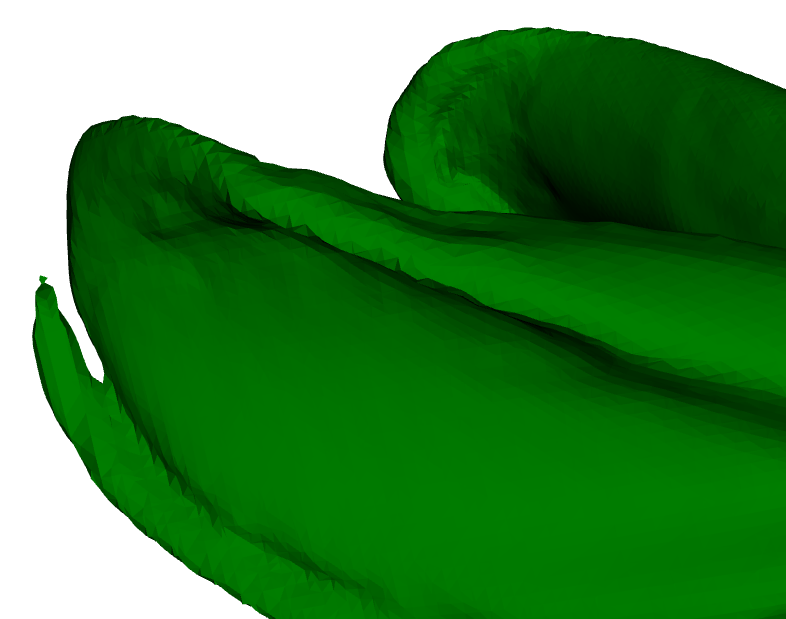
\includegraphics[max width=.5\linewidth, max height=.25\textheight, keepaspectratio]
				{img/bunny_ear}
			%\Imagen{img/bunny_ear}
			\caption[Acercamiento a la oreja derecha de \texttt{bunny}]{\label{fig:bun_ear}Acercamiento a la oreja derecha de \texttt{bunny}.}
		\end{figure}

		\begin{figure}
			%\Imagen{img/drill_drops}
			\centering
			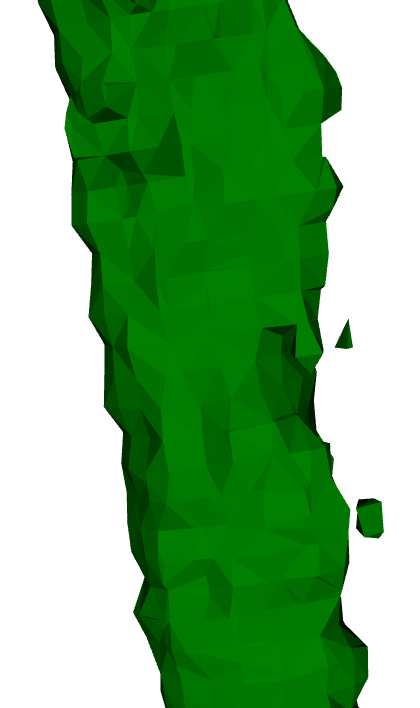
\includegraphics[max width=.5\linewidth, max height=.25\textheight, keepaspectratio]
				{img/drill_drops}
			\caption[Acercamiento a la mecha de \texttt{drill}]{\label{fig:drill_drops}Acercamiento a la mecha de \texttt{drill}. Se observan componentes inconexas con la malla principal.}
		\end{figure}

		\begin{figure}
			\centering
			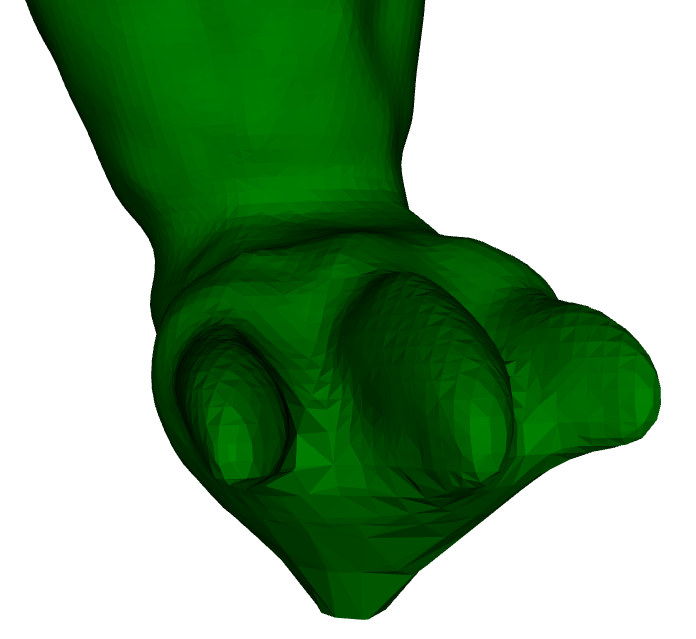
\includegraphics[max width=.5\linewidth, max height=.25\textheight, keepaspectratio]
				{img/arma_foot}
			%\Imagen{img/arma_foot}
			\caption[Acercamiento a la base de apoyo de \texttt{armadillo}]{\label{fig:base}Acercamiento a la base de apoyo de \texttt{armadillo}. Se observa un estiramiento hacia abajo debido al uso de condiciones de borde Neumann.}
		\end{figure}



	\section{Conclusiones}
		Como resultado de esta etapa se obtuvo una biblioteca de software que
		permite reconstruir un objeto tridimensional a partir de nubes
		de puntos de vistas parciales sujetas a ciertas restricciones.
		Debido al uso del método de Poisson en el rellenado, esta
		reconstrucción no presentará huecos, a excepción de la base de apoyo.

		Durante la registración, se obtuvieron resultados aceptables en casi todas las pruebas, 
		siendo uno de los fallos debido a un ángulo excesivo entre las tomas.
		Estos fallos pueden detectarse al utilizar la métrica de solapamiento y entonces proceder
		a ajustar los parámetros del algoritmo de alineación.

		A futuro se pretende desarrollar algoritmos que nos permitan relajar la
		restricción del eje de giro.
		De esta forma, se podrán combinar reconstrucciones del mismo objeto
		sobre la base de giro, con lo que se logrará recuperar la información
		perdida debido a oclusiones.

